\subsubsection{概要}
しらたまチームは1章で述べた目標のために, 
上田研究室に保存されているドキュメントを用いてロボットのセットアップや実装を行った. 
しらたまチームでは, 自己位置推定にemcl2\_ros2,ナビゲーションにnavigation2を採用した. 

%開発してないので省略
%\subsubsection{開発したパッケージ}

%システム図作成する必要あり
\subsubsection{システム構成}
ロボットに搭載した計算機,センサ,
アクチュエータの接続の関係及び計算機で実行するROS 2ノードの概要を表したものを図4に示す. 

Raspberry Piには, 車体制御のために, エンコーダと車輪駆動用のモータを接続した. 
実行するノードとしては, 
%something
がある.  


\begin{figure}[h]
  \begin{center}
    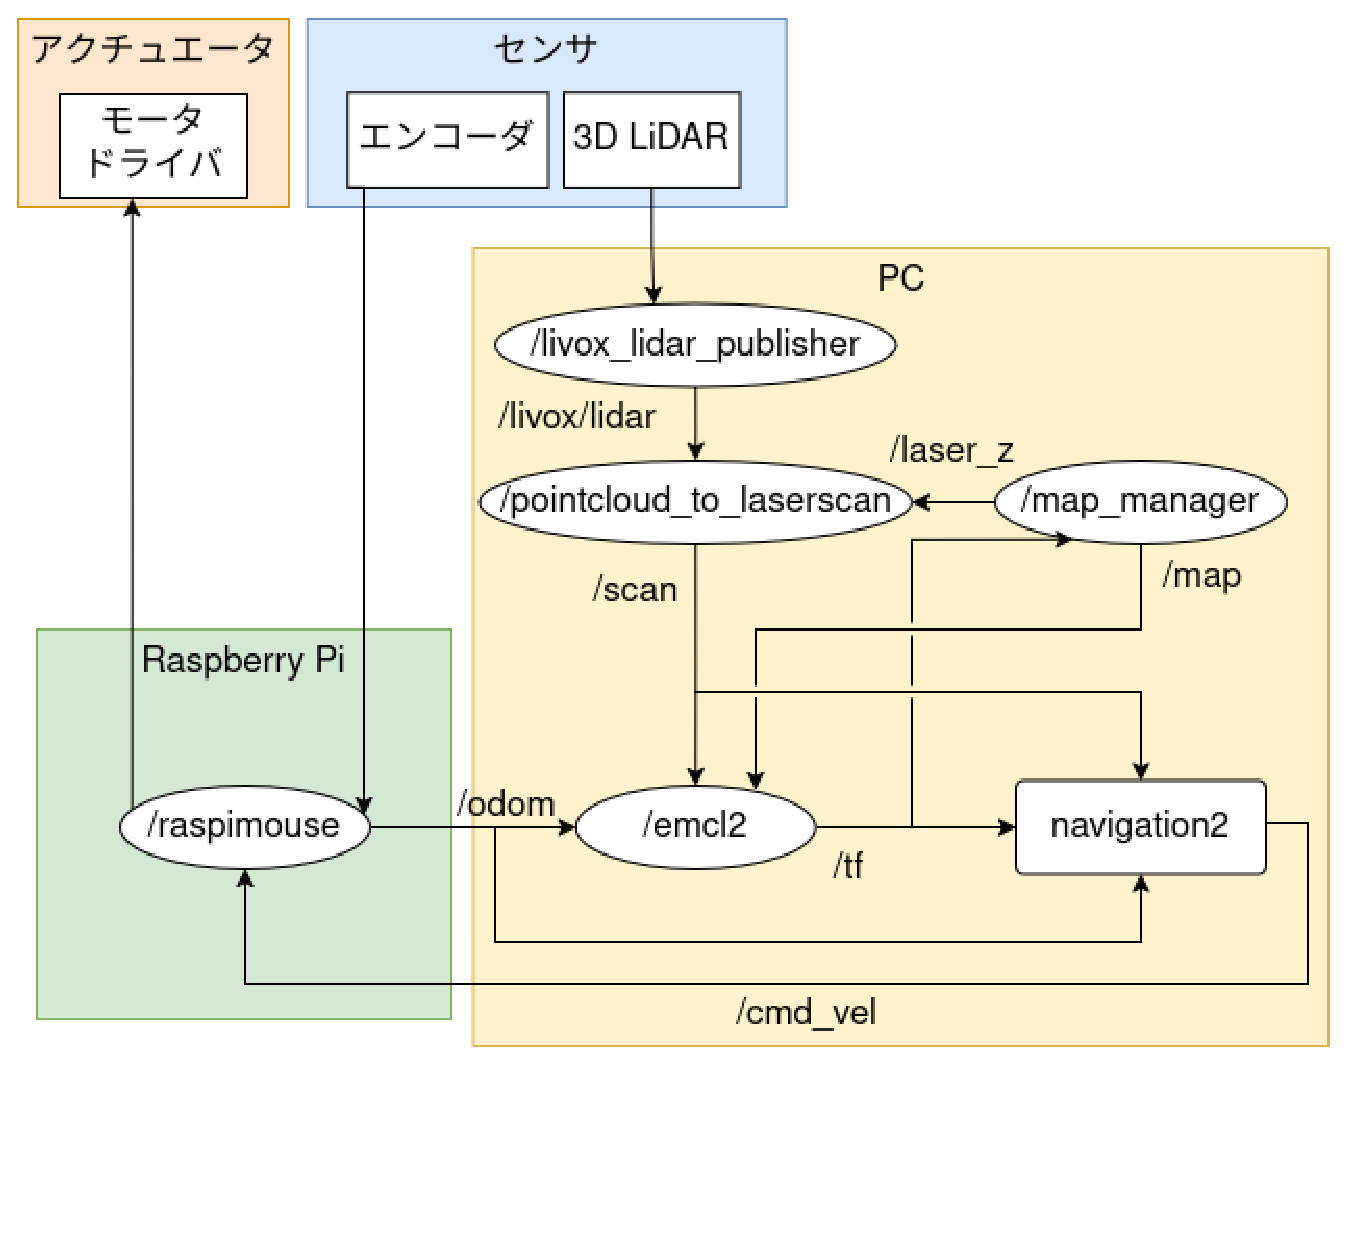
\includegraphics[width=1.0\linewidth]{figs/kinako_system_2024.eps}
    \caption{しらたまチームのシステム構成}
    \label{fig:kinako_system}
  \end{center}
\end{figure}
